\section{Method}
\label{sec:method}

Figure~\ref{fig:architecture} illustrates the overall architecture of \textsc{FinOPD}. The system operates in four stages: visual-geometric perception (\S\ref{sec:vge}), factor routing (\S\ref{sec:router}), multi-agent collaboration, and dual-track self-evolution (\S\ref{sec:opsd}, \S\ref{sec:belief}). We describe each below.
% 中文：图2展示 FinOPD 的整体架构。系统分四个阶段运行：视觉几何感知、因子路由、多智能体协作和双轨自进化。下面逐一描述。

\begin{figure*}[t]
\centering
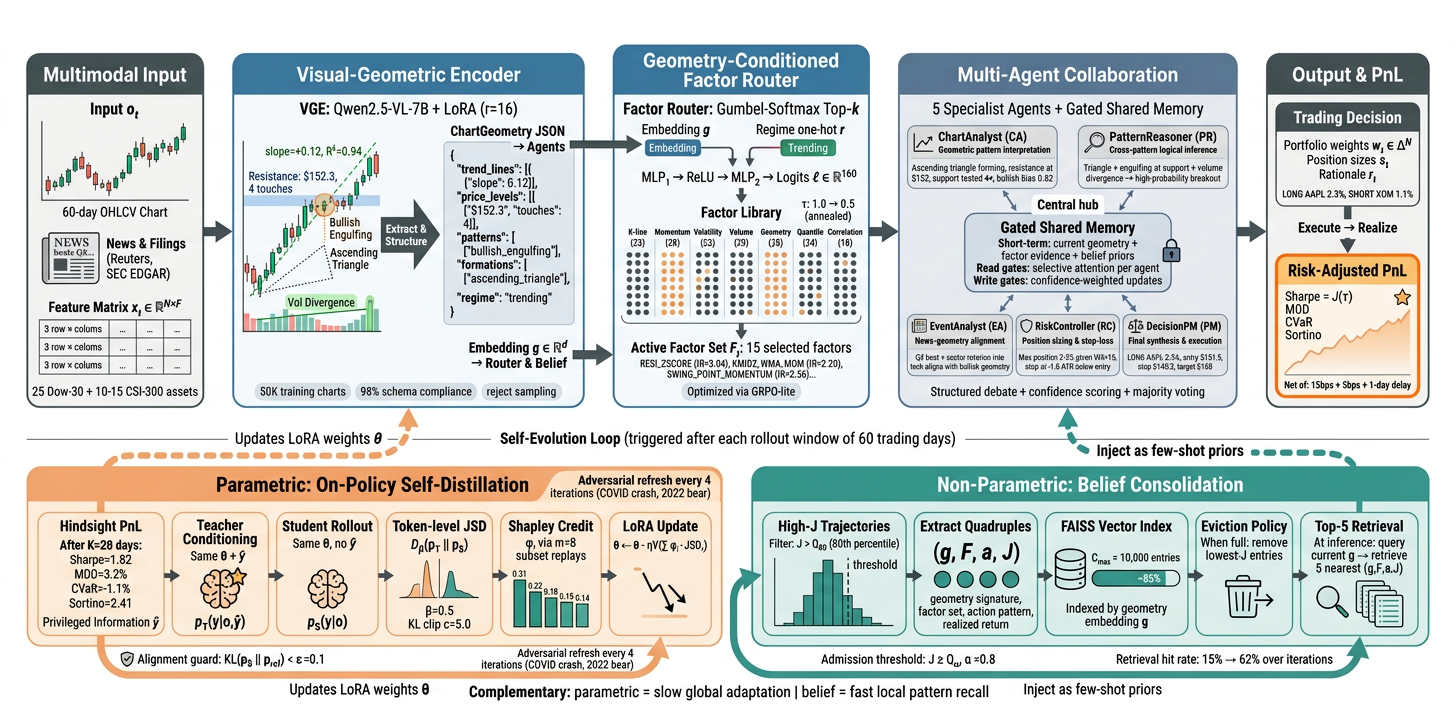
\includegraphics[width=\linewidth]{figures/fig2_framework.png}
\caption{Architecture of \textsc{FinOPD}. The Visual-Geometric Encoder extracts structured ChartGeometry from candlestick charts. The Factor Router selects 15 from 160 candidates via Gumbel top-$k$. Five specialist agents collaborate through gated shared memory. The dual-track self-evolution loop (bottom) updates LoRA parameters via on-policy self-distillation with hindsight PnL and Shapley credit (left track) and consolidates winning patterns into a belief store (right track).}
\label{fig:architecture}
\end{figure*}

\subsection{Visual-Geometric Encoder}
\label{sec:vge}

We adapt Qwen2.5-VL-7B~\cite{qwen25vl2024} with LoRA (rank 16, applied to vision encoder top layers and cross-attention modules) to output a structured \texttt{ChartGeometry} JSON containing trend lines, support-resistance levels, candlestick patterns, chart formations, volume signals, and regime state. Training data consists of approximately 50,000 US equity daily charts with weak supervision from a rule-based geometric extractor, supplemented by 1,000 human-verified samples. A JSON schema validator performs reject sampling to enforce structural compliance (target $>$98\%).
% 中文：我们用 LoRA（rank 16，作用于视觉编码器顶层和交叉注意力模块）适配 Qwen2.5-VL-7B，输出结构化 ChartGeometry JSON，包含趋势线、支撑阻力位、K线形态、图表形态、量能信号和 regime 状态。训练数据约 50,000 张美股日线图，弱监督来自规则几何提取器，辅以 1,000 张人工验证样本。JSON schema 验证器做 reject sampling 确保结构合规率 >98%。

The encoder produces two outputs: (1) structured JSON for interpretable agent reasoning, and (2) a pooled geometric embedding $\mathbf{g} \in \mathbb{R}^d$ from final-layer geometry tokens, used as the conditioning signal for the factor router and the indexing key for belief retrieval.
% 中文：编码器产生两个输出：(1) 结构化 JSON 供 agent 可解释推理；(2) 末层几何 token 的池化嵌入 g∈R^d，作为因子路由器的条件信号和 belief 检索的索引键。

\subsection{Geometry-Conditioned Factor Router}
\label{sec:router}

The factor library $\mathcal{F} = \{f_1, \ldots, f_M\}$ contains $M \approx 160$ alpha factors previously mined through LLM-driven evolutionary search, with information ratios up to 3.04 after transaction costs. The router maps the current geometric state to a factor subset via differentiable selection.
% 中文：因子库 F={f_1,...,f_M} 包含 M≈160 个通过 LLM 驱动进化搜索预挖掘的 alpha 因子，扣费后信息比率最高达 3.04。路由器通过可微选择将当前几何状态映射到因子子集。

Given the geometry embedding $\mathbf{g}$ and a regime one-hot vector $\mathbf{r} \in \{0,1\}^R$, the router computes logits $\boldsymbol{\ell} = \mathrm{MLP}_2(\mathrm{ReLU}(\mathrm{MLP}_1([\mathbf{g}; \mathbf{r}]))) \in \mathbb{R}^M$ and applies Gumbel-Softmax relaxation:
\begin{equation}
\label{eq:gumbel}
z_j = \frac{\exp((\ell_j + g_j) / \tau)}{\sum_{j'=1}^{M} \exp((\ell_{j'} + g_{j'}) / \tau)}, \quad g_j \sim \mathrm{Gumbel}(0, 1)
\end{equation}
where $\tau$ is the temperature (annealed from 1.0 to 0.5). The top-$k$ indices ($k{=}15$) from $\mathbf{z}$ yield the active factor set $F_t \subset \mathcal{F}$. Selected factors are computed and injected into the shared memory for agent consumption. The router is optimized via GRPO-lite within the self-evolution loop (\S\ref{sec:opsd}).
% 中文：给定几何嵌入 g 和 regime one-hot 向量 r，路由器计算 logits 并应用 Gumbel-Softmax 松弛。温度 τ 从 1.0 退火到 0.5。从 z 中取 top-k（k=15）索引得到活跃因子集 F_t⊂F。选中因子被计算并注入共享记忆供 agent 消费。路由器通过自进化循环中的 GRPO-lite 优化。

\subsection{On-Policy Self-Distillation with Hindsight PnL}
\label{sec:opsd}

We enable the same model to serve as both student and teacher through differential conditioning (Figure~\ref{fig:opsd}). The student reasons from current observations; the teacher additionally conditions on realized risk-adjusted returns as privileged information.
% 中文：我们通过差异条件化使同一模型同时充当学生和教师。学生从当前观测推理；教师额外条件化于已实现的风险调整收益作为特权信息。

\begin{figure}[t]
\centering
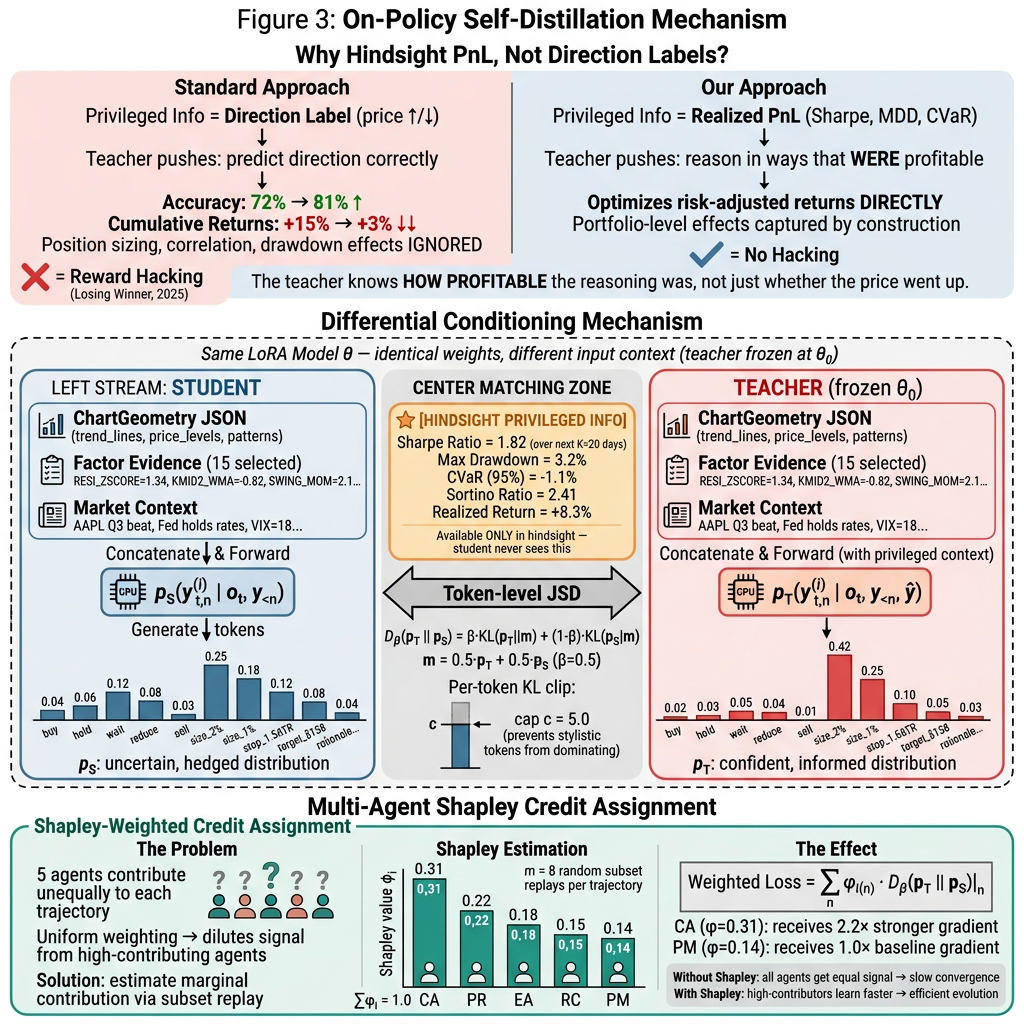
\includegraphics[width=\linewidth]{figures/fig3_mechanism.png}
\caption{On-policy self-distillation. The same LoRA model defines student (conditioned on $o_t$) and teacher (conditioned on $o_t$ plus hindsight PnL). Token-level JSD with Shapley weighting drives parametric evolution.}
\label{fig:opsd}
\end{figure}

\paragraph{Formulation.} Let $o_t$ denote the observation at time $t$. Agent $i$ produces a sequence $y^{(i)}_t = (y^{(i)}_{t,1}, \ldots, y^{(i)}_{t,L})$. The shared LoRA parameters define:
\begin{align}
p_S(y^{(i)}_{t,n} \mid o_t, y^{(i)}_{t,<n}) &\quad \text{(student)} \\
p_T(y^{(i)}_{t,n} \mid o_t, y^{(i)}_{t,<n}, \hat{y}) &\quad \text{(teacher)}
\end{align}
where $\hat{y}$ is the privileged information: realized risk-adjusted returns (Sharpe, MDD, CVaR, Sortino) over the subsequent $K{=}20$ trading days, serialized as a token sequence prepended to the teacher's prompt. Teacher weights are frozen to the initial checkpoint.
% 中文：设 o_t 为 t 时刻观测。Agent i 产生序列 y^(i)_t。共享 LoRA 参数定义学生策略（仅条件于 o_t）和教师策略（额外条件于特权信息 ŷ）。ŷ 是后续 K=20 个交易日的已实现风险调整收益（Sharpe、MDD、CVaR、Sortino），序列化为 token 序列前置到教师 prompt。教师权重冻结为初始 checkpoint。

\paragraph{Training objective.} At each token position, we minimize the generalized Jensen-Shannon divergence:
\begin{equation}
D_\beta(p_T \| p_S) = \beta \, \mathrm{KL}(p_T \| m) + (1{-}\beta) \, \mathrm{KL}(p_S \| m), \quad m = \beta \, p_T + (1{-}\beta) \, p_S
\end{equation}
with per-token KL clipping to prevent stylistic tokens from dominating:
\begin{equation}
\mathrm{KL}_{\mathrm{clip}}(n) = \sum_{v=1}^{V} \min\left( p_T(v|n) \log \frac{p_T(v|n)}{p_S(v|n)},\; c \right)
\end{equation}
% 中文：在每个 token 位置最小化广义 Jensen-Shannon 散度，并用逐 token KL 裁剪防止风格性 token 主导梯度。每个词表项在每个位置的 KL 贡献被限制在上限 c 以内。

\paragraph{Shapley credit assignment.} For each high-reward trajectory, we sample $m{=}8$ random agent subsets and perform leave-subset-out replay to estimate marginal contributions $\phi_i$. The normalized Shapley values weight the distillation loss per agent, preventing dilution across unevenly contributing agents.
% 中文：对每条高奖励轨迹，随机采样 m=8 个 agent 子集做 leave-subset-out 重放以估计边际贡献 φ_i。归一化 Shapley 值加权每个 agent 的蒸馏损失，防止在贡献不均的 agent 之间稀释学习信号。

\paragraph{GRPO-lite for the router.} Factor selection is a discrete action optimized separately. Within each mini-batch, the advantage of trajectory $j$ is $(J_j - \bar{J})$, requiring no critic network.
% 中文：因子选择是离散动作，单独优化。每个 mini-batch 内，轨迹 j 的优势为 (J_j - J̄)，不需要 critic 网络。

\paragraph{Alignment guard.} We maintain $\mathrm{KL}(p_S \| p_{\mathrm{ref}}) < \epsilon$ against the reference policy. Every four iterations, adversarial samples from regime-shift periods (2020 COVID crash, 2022 bear market) provide off-policy refresh.
% 中文：维持学生对参考策略的 KL 散度 < ε。每四轮迭代，用 regime 转换时期（2020 COVID 崩盘、2022 熊市）的对抗样本做离线策略刷新。

The complete self-evolution loop is summarized in Algorithm~\ref{alg:finopd}.

\begin{algorithm}[t]
\caption{\textsc{FinOPD} Self-Evolution (One Iteration)}
\label{alg:finopd}
\begin{algorithmic}[1]
\REQUIRE Student $p_S(\theta)$, frozen teacher $p_T(\theta_0)$, router $\pi_R$, belief store $\mathcal{B}$, window $\mathcal{W}$
\FOR{each day $t \in \mathcal{W}$}
\STATE $\mathbf{g}_t \leftarrow \mathrm{VGE}(I_t)$; retrieve priors from $\mathcal{B}$ via $\mathbf{g}_t$
\STATE $F_t \leftarrow \pi_R(\mathbf{g}_t, \mathrm{regime}_t)$ \hfill $\triangleright$ Gumbel top-$k$
\FOR{agent $i = 1 \ldots 5$}
\STATE $y^{(i)}_t \sim p_S(\cdot \mid o_t, F_t)$
\ENDFOR
\ENDFOR
\STATE $J \leftarrow \mathrm{RiskAdjPnL}(\tau)$; \ $\hat{y} \leftarrow \mathrm{serialize}(J)$
\STATE Compute $p_T(\cdot \mid o, y_{<n}, \hat{y})$ at all positions
\STATE $\{\phi_i\} \leftarrow \mathrm{ShapleyCredit}(\tau, m{=}8)$
\STATE $\mathcal{L} \leftarrow \sum_n \phi_{i(n)} \cdot D_\beta(p_T \| p_S)|_n$ with per-token KL clip
\STATE $\theta \leftarrow \theta - \eta \nabla_\theta \mathcal{L}$; \ update $\pi_R$ via GRPO-lite
\IF{$J > Q_{80}(\text{history})$}
\STATE Insert $(\mathbf{g}, F, a, J)$ into $\mathcal{B}$
\ENDIF
\IF{$\mathrm{KL}(p_S \| p_\mathrm{ref}) > \epsilon$}
\STATE Rollback $\theta$ to last safe checkpoint
\ENDIF
\RETURN Updated $\theta$, $\pi_R$, $\mathcal{B}$
\end{algorithmic}
\end{algorithm}

\subsection{Long-Term Belief Consolidation}
\label{sec:belief}

Parametric updates capture distributional drift but gradually dilute recurring concrete patterns through averaging. We maintain a non-parametric belief store to preserve pattern specificity.
% 中文：参数更新捕捉分布漂移但通过平均逐渐稀释反复出现的具体模式。我们维护非参数 belief 存储以保留模式特异性。

From high-reward trajectories ($J$ above the 80th percentile), we extract quadruples $(\mathbf{g}, F, a, J)$: geometry signature, selected factor set, action pattern, and realized return. These are indexed by $\mathbf{g}$ in a FAISS vector store with capacity constraints:
\begin{equation}
|\mathcal{B}| \leq C_{\max}, \quad \forall\, (\mathbf{g}, F, a, J) \in \mathcal{B}: \; J \geq Q_{\alpha}(\{J_i\}_{i=1}^{|\mathcal{B}|})
\end{equation}
where $C_{\max} = 10{,}000$ and $\alpha = 0.8$. When capacity is reached, lowest-$J$ entries are evicted. At inference, the current geometry signature retrieves top-5 nearest neighbors, and the associated $(F, a)$ pairs are injected as few-shot priors into the shared memory.
% 中文：从高奖励轨迹（J 高于 80 分位）中抽取四元组 (g, F, a, J)：几何签名、选中因子集、动作模式和已实现收益。这些按 g 索引在 FAISS 向量存储中，受容量约束：|B|≤C_max=10,000 且 J≥Q_0.8。达到容量时驱逐最低 J 的条目。推理时，当前几何签名检索 top-5 近邻，关联的 (F, a) 对作为 few-shot 先验注入共享记忆。

The parametric track adjusts how the model reasons across all situations (slow, global). The belief store provides what to do in specific situations (fast, local). In ablations (\S\ref{sec:experiments}), we show that neither track alone matches their combination.
% 中文：参数轨道调整模型在所有情况下如何推理（慢、全局）。Belief 存储提供在特定情况下做什么（快、局部）。消融实验中我们展示单独任一轨道都不如两者组合。
